\documentclass{beamer}
\usepackage[english,russian]{babel}
\usepackage[utf8]{inputenc}
\usetheme{Warsaw}
\begin{document}
\title{Параметры фотонных орбит вблизи скалярных черных дыр}
\subtitle{Выпускная квалификационная работа}
\author{Автор: Трофимов Аркадий Александрович \\
Научный руководитель:
д. ф.-м. н. Цирулёв А.Н.
}
\institute{Тверской государственный университет}
\date{Тверь, 2020}
% Создание заглавной страницы
\frame{\titlepage}
% Автоматическая генерация содержания
\frame{\frametitle{Цели и задачи работы}

1. Изучить движение частиц в пространстве-времени Шварцшильда.

2. Изучить и описать движение фотонов вблизи скалярной черной дыры.
}
\frame{\frametitle{Решение шварцшильда}
    Метрика Шварцшильда
\begin{equation}\label{1.1}
     ds^2=A dt^2- \frac{dr^2}{B}  - r^2(d\theta^2 + \sin^2\theta d\varphi^2)
\end{equation}
где метрическая функции $A$ и $B$ зависят только от радиальной координаты $r$ и $A$ и $B$ равны между собой. В метрике Шварцшильда
\begin{equation}
    A=1-\frac{2m}{r},
\end{equation}
где $m$ -- масса притягивающего объекта.
}
\frame{\frametitle{Уравнение геодезической и интегралы движения}
Движение по геодезической описывется лагранжианом
\begin{equation}{\label{1.3}}
    \mathscr{L} = A\left(\frac{dt}{d\tau}\right)^2 - A^{-1}\left(\frac{dr}{d\tau}\right)^2 - r^2\left(\frac{d\theta}{d\tau}\right)^2 - r^2 \sin^2 \theta \left(\frac{d\varphi}{d\tau}\right)^2,
\end{equation}
и него вычисляются интегралы движения
\begin{gather}
    \label{3}
    A\frac{dt}{d\tau} = E, \ \ \ \
    r^2 \frac{d\varphi}{d\tau} = J,\\
    \label{4}
    \left(\frac{dr}{d\tau} \right)^2 = E^2 - V_{eff},
\end{gather}
где $V_{eff}$ -- эфективный потенциал, заданный формулой
\begin{equation}
    V_{eff} = A\left(k+\frac{J^2}{r^2}\right),
\end{equation}
}
\frame{\frametitle{Орбиты в пространстве-времени Шваршильда}
Одним из главных параметров определения орбиты является угол между её перицентрами
\begin{equation}
    \left(\frac{dr}{d\varphi}\right) = \frac{r^2}{J} \sqrt{E^2 - V_eff}.
\end{equation}
Интегрируя последние вырожение, мы получим колебания угол орбиты $\widetilde{\varphi}$
\begin{equation}
    \widetilde{\varphi}^{Sch} = J\int_{r_{min}} ^{r_{max}} \frac{dr}{r^2 \sqrt{E^2 - V_{eff}}},\ \ \ \ \
\end{equation}
Также, можно вычислить период колебаний, радиальную и орбитальную скорости
\begin{gather}
    \widetilde{T}^{Sch} = E \int_{r_{min}}^{r_{max}} \frac{dr}{A \sqrt{E^2 - V_{eff}}} ,\\
    \omega^{Sch}  = \frac{J}{E} \frac{A}{r^2},\ \ \
    v^{Sch} = \frac{dr}{dt} = \frac{A}{E} \sqrt{E^2 - V_{eff}}.
\end{gather}
}
\frame{\frametitle{Математическая модель скалярной черной дыры}
Рассмотрение скалярной черной дыры начнем с действия
\begin{equation}
    \Sigma = \frac{1}{8\pi} \int \left(-\frac{1}{2} R  + (d\phi,d\phi) - 2V(\phi)\right)\sqrt{|g|}d^4x,
    \nonumber
\end{equation}
которое в координатах Шварцшильда примет вид
\begin{equation}{\label{2.1}}
    ds^2 = Adt^2 - \frac{dr^2}{B} - r^2d\theta^2 - r^2\sin^2\theta d\varphi^2,
\end{equation}
где представим функцию $A$ в виде
\begin{equation}
    A(r) = B(r) e^{2F(r)}.
\end{equation}
}
\frame{\frametitle{Основные функции модели скалярной черной дыры}
Основные функции математической модели возьмем из ~\cite{Potashov2019}
\begin{equation}{\label{2.7}}
    F(r) = - \int_r^{\infty} \phi'^2 rdr.
\end{equation}
\begin{gather}
    \label{2.8}
    \xi = r + \int_r^{\infty} (1-e^F) dr,\\
    \label{2.9}
    A(r) = 2r^2 \int_r^{\infty} \frac{\xi - 3m}{r^4} e^F dr, \ \
    B(r) = e^{-2F} A, \\
    \label{2.10}
    \widetilde{V}(r) = \frac{1}{2r^2}\left(1- 3B + r^2 \phi'^2 B + 2e^{-F} \frac{\xi - 3m}{r}\right).
\end{gather}
}
\frame{\frametitle{Эффективный потенциал для безмассовых частиц}
Так как для фотона $k=0$, то формула эффективного потенциала примет вид
\begin{equation}
    V_{eff} = A\frac{J^2}{r^2}.
\end{equation}
где $E$ -- удельная энергия, $J$ -- удельный угловой момент частицы.
\begin{center}
    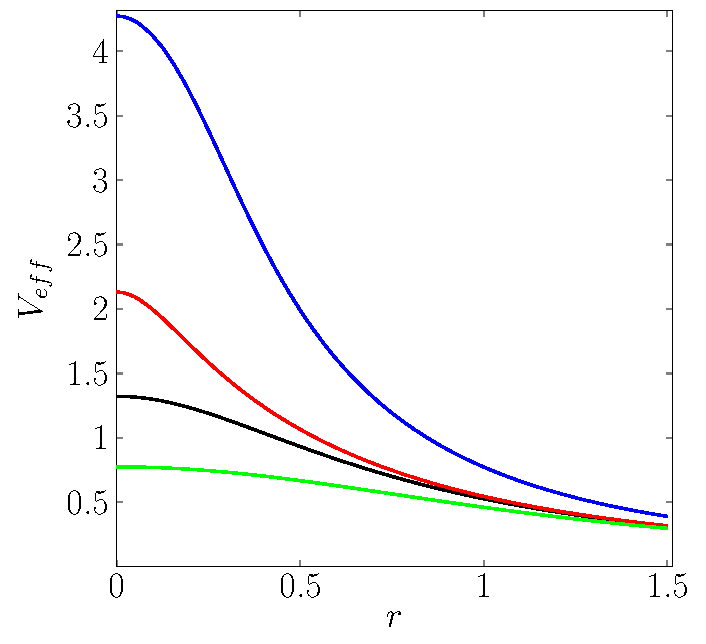
\includegraphics[width=7cm]{fig_1.pdf}
\end{center}
графики эффективных потенциалов безмассовых геонов для фотонных орбит.
}
\frame{\frametitle{Параметры орбит}
Далее путем несложных преобразований получим основные параметры для орбит фотонов
\begin{gather}
     \label{2.16}
    \widetilde{T}^{shb} = E \int_{r_{min}}^{r_{max}} \frac{e^F}{A \sqrt{E^2 - V_{eff}}} dr,\\
    \label{2.17}
    \omega^{sbh}  = \frac{J}{E} \frac{A}{r^2},\ \ \
    v^{sbh} = \frac{dr}{dt} = \frac{A e^{-F}}{E} \sqrt{E^2 - V_{eff}}.
\end{gather}
\begin{center}
    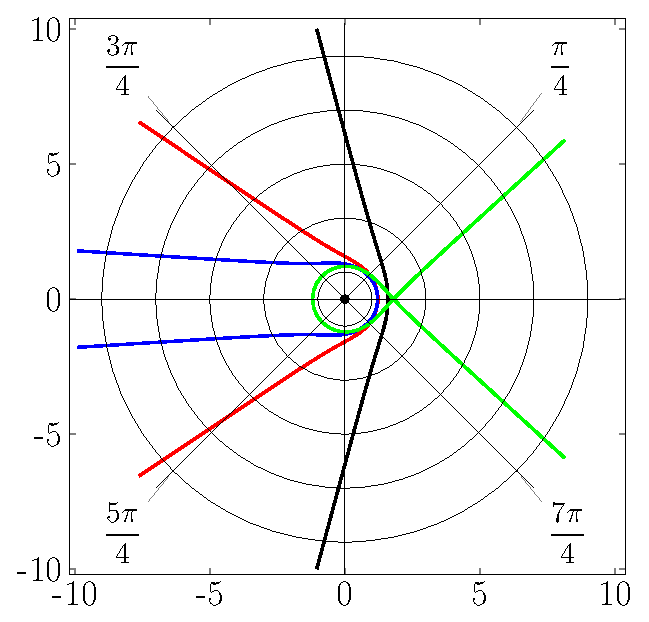
\includegraphics[width=1.4in]{fig_4.pdf}
\end{center}
Фотонные орбиты для разных значений $E^2 \in (0,1)$
}
\frame{\frametitle{Численные выводы}
С помошью простых преобразований получим параметры в виде
\begin{equation}
    e^{F} = 1 - a - \frac{2a}{7}r^3, \ \ \
    0\leq r \leq 1,
    \nonumber
\end{equation}
и
\begin{equation}
    e^{F} = 1 -  \frac{2a}{r^3} - \frac{9a}{7r^4}, \ \ \
    1 \leq r < \infty,
\end{equation}
\begin{center}
    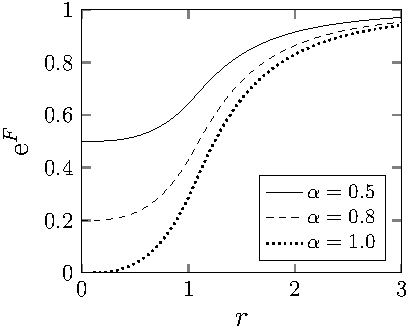
\includegraphics[width=1.4in]{figure1a.pdf}
    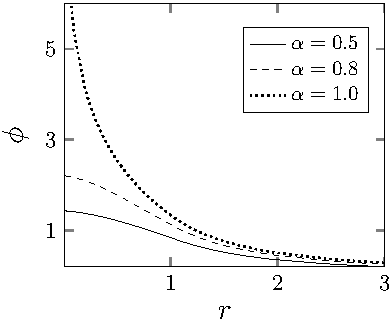
\includegraphics[width=1.4in]{figure1b.pdf}
\end{center}
'Cкалярный заряд' $ e^F $ является строго монотонной функцией ($ e^F \rightarrow 1 $ слева при $ r\rightarrow \infty $) и однозначно определяет соответствующую полевую функцию $\phi$.
}
\frame{\frametitle{Численные выводы}
Далее находим
\begin{equation}
    \xi = \frac{3a}{2} + (1-a)r + \frac{a}{14} r^4, \ \ \
    0 \leq r \leq 1,
    \nonumber
\end{equation}
\begin{equation}
    \xi = r +\frac{a}{r^2} - \frac{3a}{7r^3}, \ \ \
    1 \leq a < \infty.
    \nonumber
\end{equation}
И метрическую функцию $A$
\begin{multline}
     A = -\frac{(1-a)(2m-a)}{r} + (1-a)^2 +\\+ \left(\frac{6}{7}(2m-a)\ln r +
     + \frac{8}{5} - \frac{88}{105}a - \frac{54}{49}\right)
     ar^2 -
     - \frac{5}{7}a(1-a)r^3 -\frac{a^2}{98}r^6 , \\ 0 \leq r \leq 1,
     \nonumber
\end{multline}
}
\frame{\frametitle{Численные выводы}
\begin{multline}
     A = 1 -\frac{2m}{r} - \frac{2a}{5r^2} + \left(m + \frac{1}{7}\right)\frac{2a}{r^4} - \frac{54am}{49r^5} - \frac{a^2}{2r^6} + \frac{10a^2}{21r^7} - \frac{27a}{245r^8}, \\
     1\leq r < \infty,
\end{multline}
Напомним, что $B=f= A e^{e^F}$
\begin{center}
    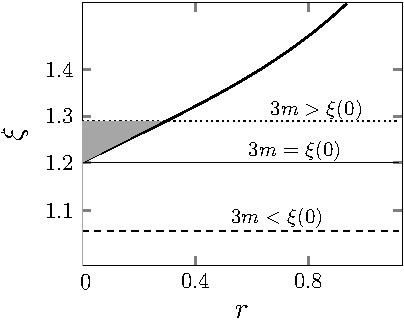
\includegraphics[width=1.8in]{figure2a.pdf}
    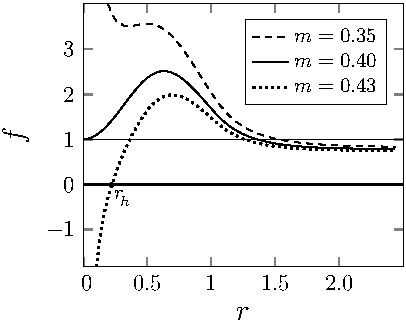
\includegraphics[width=1.8in]{figure2b.pdf}
\end{center}
}
\frame{\frametitle{Численные выводы}
Подставляя полученные результаты в (\ref{2.16}) и (\ref{2.17}) получим
\begin{gather}
    \omega^{sbh} = \left(\frac{6}{7} (2m-1)\ln r + \frac{1}{3} - \frac{12m}{49} - \frac{3r^4}{98}\right)^{1/2}
\end{gather}
\begin{equation}
    v^{sbh} = \frac{3}{r} \left((2m-1)\ln r + \frac{8}{9} - \frac{9m}{7} - \frac{r^4}{84} \right).
\end{equation}
\begin{center}
    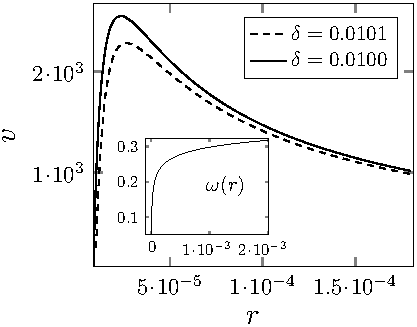
\includegraphics[width=1.5in]{figure5a.pdf}
    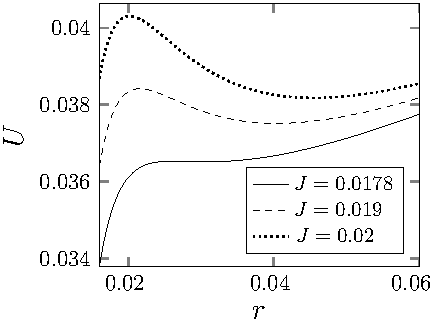
\includegraphics[width=1.5in]{figure5b.pdf}
\end{center}
Радиальная скорость пробной частицы, падающей к цен-тру крайней черной дыры с $ a = 1 $ и $ m = 1/2 + \delta $ вблизи ее горизонта;на вставке показана угловая частота орбиты.
}


\frame{\frametitle{Литература}
\begin{thebibliography}{99}

\bibitem{Chandrasekar}
Чандрасекар С. Математическая теория чёрных дыр.
М.: Наука, 1989.

\bibitem{Potashov2019}
I.M. Potashov, Ju.V. Tchemarina and A.N. Tsirulev. Bound orbits near black holes with scalar hair. Journal of Physics, V. 1390, No 1, 012097 (2019)

\bibitem{Solovyev2012}
D.A. Solovyev, A.N. Tsirulev, General properties and exact models of static selfgravitating scalar field configurations. Class. Quantum Grav. \textbf{29}, 055013 (2012)
\end{thebibliography}

}
\end{document} 